% Preamble
\documentclass[a4paper, 12pt]{article}
\usepackage[margin=1in]{geometry} % Set margin
\usepackage{pdfpages} % Insert pdf pages
\usepackage{amssymb,amsmath,amsthm, amsfonts} % Math libraries

% Custom commands
\newcommand{\sub}[1]{\subsection{\underline{#1}}}
\newcommand{\subsub}[1]{\subsubsection{\underline{#1}}}
\newcommand{\?}{\stackrel{?}{=}}
\newcommand{\R}{\ensuremath{\mathbb{R}}}
\newcommand{\F}{\ensuremath{\mathbb{F}}}
\newcommand{\N}{\ensuremath{\mathbb{N}}}
\newcommand{\Onef}{\ensuremath{1_{\F}}}
\newcommand{\Zerof}{\ensuremath{0_{\F}}}
\newcommand{\eqbcuz}[1]{\text{~$\stackrel{(#1)}{=}$~}}
\newcommand{\eq}[1]{\begin{align*}#1\end{align*}}
\newcommand{\eqn}[1]{\begin{align}#1\end{align}}
\renewcommand{\qed}{$$\blacksquare$$}
\renewcommand{\b}[1]{\textbf{#1}}
\renewcommand{\because}[1]{~\b{(#1)}\\}
\renewcommand{\d}{\ensuremath{\Downarrow\\~}}
\newtheorem{lemma}{Lemma}

% Begin Document %
\begin{document}

% Title Page
\begin{titlepage}
    %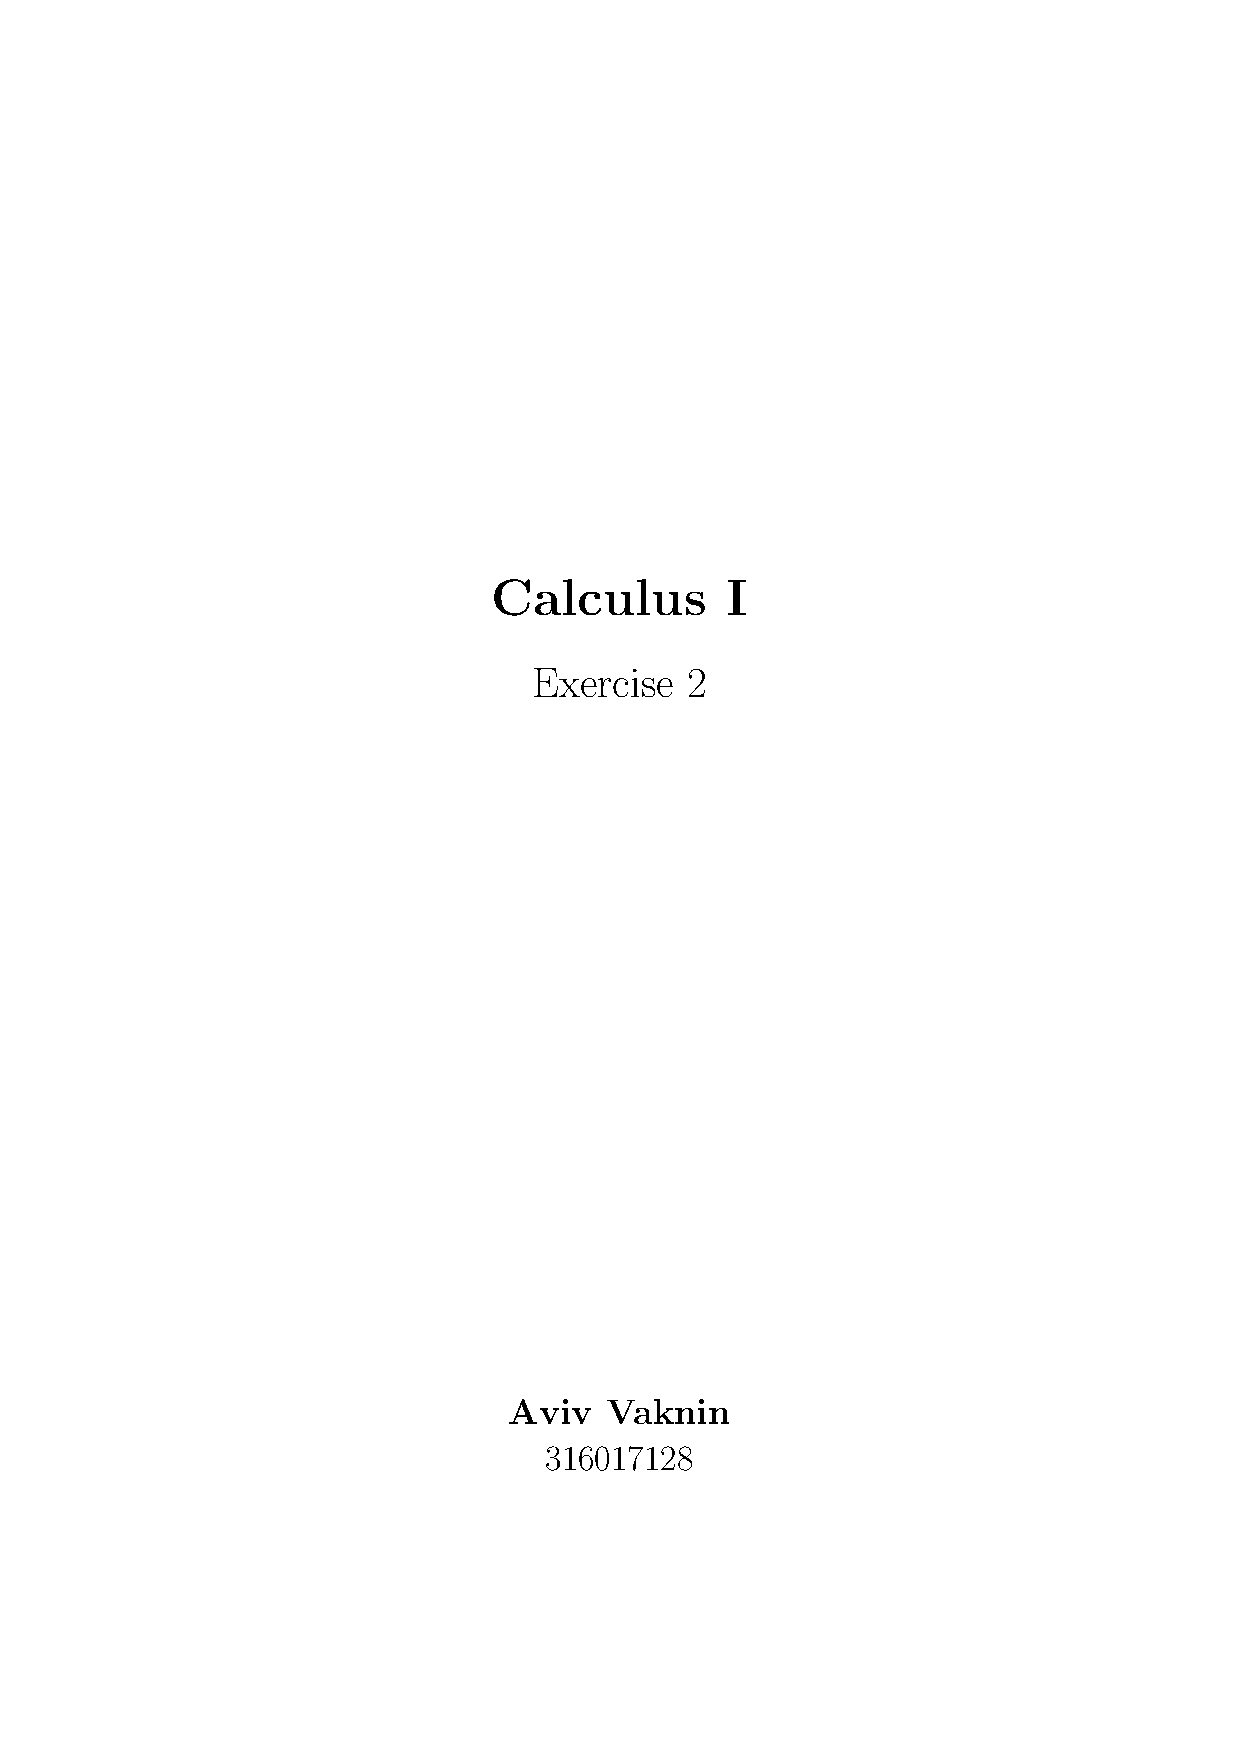
\includepdf{title.pdf}
\end{titlepage}

%1
\section{Prove that \eq{a\leq{b} \iff \forall\epsilon>0~~a<b+\epsilon}}
\sub{$ a\leq{b} \Rightarrow \forall\epsilon>0~~a<b+\epsilon $:}
It is given that: \eq{0<\epsilon && a\leq{b}}
Therefore, because according to axiom $O3$ an ordered field is adhering to addition:
\eq{a+0<b+\epsilon}
It is worth mentioning that due to the uniqueness of zero, $b+\epsilon$ must be \textit{greater} than zero, rather than greater than or \textit{equal} to zero.
\sub{$ a\leq{b} \Leftarrow \forall\epsilon>0~~a<b+\epsilon $:}
We'll rephrase using contraposition: \eq{a>b \Rightarrow \exists\epsilon>0~~a\geq{b+\epsilon}}
We need to find an $\epsilon>0$ so that $a\geq{b+\epsilon}$.\\
Let $\epsilon=a-b$, now, we can see that:
\eq{
    b+\epsilon &= b+(a-b) = a\\
    a&\geq{b+\epsilon}
}
\qed

%2
\section{Prove that \eq{\forall{m,n}\in{\mathbb{N}}~~mn\in{\mathbb{N}}}}
Let's assume that $m$ is some arbitrary natural number.\\
We'll prove using induction, starting with $n=1$:
According to axiom \textit{M3}:
\eq{m\cdot{1}=m}
It is given that $m\in{\mathbb{N}}$, therefore this case is valid.
Now, let's assume that it is true for a general $n$, i.e. $n=n$, and:
\eq{mn\in{\mathbb{N}}}
Now, we'll check $n=n+1$:
According to axiom \textit{D}:
\eq{ m(n+1)=mn+m }
We've assumed that $mn\in{\mathbb{N}}$, and it is given that $m\in{\mathbb{N}}$.\\
In addition, we've shown in exercise \textit{2a} that the natural numbers adhere to addition.\\
Therefore: \eq{mn\in{\mathbb{N}},~m\in{\mathbb{N}}\implies(mn+m)\in{\mathbb{N}}}
\qed

%3
\section{Prove the following:}
\sub{Prove:}
\eq{\sum^{n}_{k=1}k^{2}=\frac{n(n+1)(2n+1)}{6}}
We'll prove this by induction.
\subsub{$n=1$}
we can see that the statement is true for $n=1$:
\eq{\sum^{1}_{k=1}k^{2}\eqbcuz{def}1^2=\frac{1(1+1)(2+1)}{6}}
\subsub{$n=n$}
Now, we'll assume it is true for $n=n$, i.e.:
\eq{\sum^{n}_{k=1}k^{2}\eqbcuz{def}1^2+2^2+...+n^2=\frac{n(n+1)(2n+1)}{6}}
\subsub{$n=n+1$}
And now, we'll check $n=n+1$:
\eq{\sum^{n+1}_{k=1}k^{2}\eqbcuz{def}1^2+2^2+...+n^2+(n+1)^2=\frac{(n+1)(n+2)(2(n+1)+1)}{6}}
Now, according to the definition: \eq{ \sum^{n}_{k=1}k^{2}+(n+1)^2 = \sum^{n+1}_{k=1}k^{2} }
Therefore, we need to check if: \eq{\frac{n(n+1)(2n+1)}{6}+(n+1)^2=\frac{(n+1)(n+2)(2(n+1)+1)}{6}}
And after solving each side, we receive: \eq{0=0}
Therefore, we've proved that the statement is true for $n=n+1$.
\qed

\sub{Prove:}
\eq{\sum^{n-1}_{i=0}x^{i}=\frac{\Onef-x^n}{\Onef-x}}
\b{Note}: I'll use $\Onef$ and $1$ interchangeably while proving this.\\
We'll prove this by induction.
\subsub{$n=1$}
we can see that the statement is true for $n=1$, because by definition, $a^0=1$:
\eq{\sum^{0}_{i=0}x^{i}\eqbcuz{def}x^0=\frac{\Onef-x^1}{\Onef-x}=\frac{\Onef-x}{\Onef-x}=1}
\subsub{$n=k$}
Now, let's assume that the statement is true for $n=k$, i.e.:
\eq{\sum^{k-1}_{i=0}x^{i}\eqbcuz{def}1+x+x^2...+x^{k-1}=\frac{\Onef-x^k}{\Onef-x}}
\subsub{$n=k+1$}
\eq{\sum^{k}_{i=0}x^{i}\eqbcuz{def}1+x+x^2...+x^{k-1}+x^k=\frac{\Onef-x^{k+1}}{\Onef-x}}
According to the definition:
\eq{ \sum^{k-1}_{i=0}x^{i} + x^k = \sum^{k}_{i=0}x^{i} }
Therefore, we need to prove that:
\eq{ \frac{\Onef-x^k}{\Onef-x} + x^k = \frac{\Onef-x^{k+1}}{\Onef-x} }
\eq{
    \frac{\Onef-x^k}{\Onef-x} + x^k =
    \frac{\Onef-x^k+(\Onef-x)x^k}{\Onef-x} =
    \frac{\Onef-x^k+x^k-x^{k+1}} {\Onef-x} =
    \frac{\Onef-x^{k+1}} {\Onef-x}
}
Thus, we've proved that:
\eq{ \sum^{k-1}_{i=0}x^{i} + x^k = \sum^{k}_{i=0}x^{i} }
\qed

\section{\eq{ m,n,s,t\in{\F}~~n,t>0}Prove: \eq{\frac{m}{n}<\frac{s}{t}\implies \frac{m}{n}<\frac{m+s}{n+t}<\frac{s}{t} }}
?\pagebreak

%7
\setcounter{section}{7}
\section{\eq{ x,y\geq{0},~n\in{\N}} Prove: \eq{x<y \iff x^n<y^n }}
\sub{$x<y \implies x^n<y^n$}
\begin{lemma}
    \eq{
        a,b,c,d > 0\\
        a>b,~c>d
    }
    Because $a>b$, we can multiply both by c, which is positive:
    \eq{ac>bc}
    Similarly: \eq{bc>bd}
    Therefore, due to transitivity: \eq{bd<bc<ac}
    \qed
\end{lemma}
~\\We'll prove this by induction.
\subsub{$n=1$}
By definition, $a^1=a$, therefore we can see the statement is true for n=1:
\eq{ x^1=x<y=y^1 }
\subsub{$n=k$}
Let's assume it is true for $n=k$, that is:
\eq{x<y \implies x^k<y^k}
\subsub{$n=k+1$}
\eq{
    x&<y\\
    x^{k+1}&=x^k\cdot{x}\\
    y^{k+1}&=y^k\cdot{y}
}
According to our $n=k$ assumption:
\eq{x^k<y^k}
Therefore, because it is given that $x,y\geq{0}$, and \textit{Lemma 1}, we can show that:
\eq{x^{k+1}=x^{k}x<y^{k}y=y^{k+1}}
We've shown: \eq{x<y \implies x^n<y^n}
\sub{$x<y \impliedby x^n<y^n$}
The contrapositive form of this assertion is:
\eq{x\geq{y}\implies{x^n\geq{y^n}}}
Similarly to how we proved the $\implies$ part, we'll prove it by induction:
\subsub{$n=1$}
We can easily see that this is correct, as $a^1=a$: \eq{x^1=x\geq{y}=y^1}
\subsub{$n=k$}
Let's assume it is true for $n=k$, that is:
\eq{x\geq{y} \implies x^k\geq y^k}
\subsub{$n=k+1$}
\eq{
    x&\geq y\\
    x^{k+1}&=x^k\cdot{x}\\
    y^{k+1}&=y^k\cdot{y}
}
According to our $n=k$ assumption:
\eq{x^k\geq{y^k}}
Therefore, because it is given that $x,y\geq{0}$, and \textit{Lemma 1}, we can show that:
\eq{x^{k+1}=x^{k}x\geq y^{k}y=y^{k+1}}
We've shown: \eq{x\geq{y} \implies x^n\geq{y^n}}
\qed

% End
\end{document}